\subsection{Instruction for legacy GBTx programmer}
\label{appx:legacy-gbtx-programmer}

A typical UI of legacy GBTx programmer is shown in
\autoref{fig:gbtx-programmer-ui-old}

\begin{figure}[!ht]
	\centering
	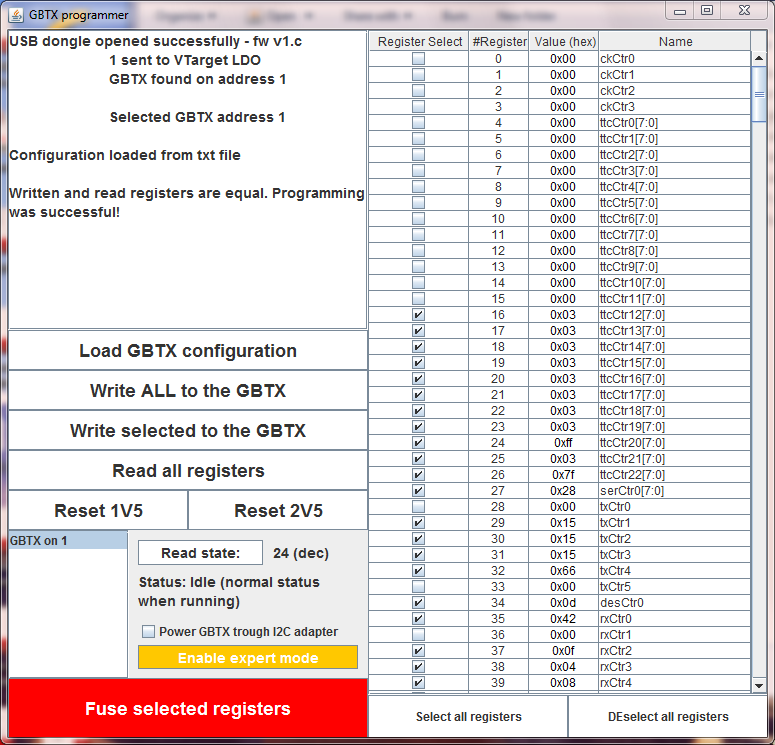
\includegraphics[width=0.9\textwidth]{res/gbtx_programmer_v1_ui.png}
	\caption{Main UI of GBTX programmer, version 1.}
	\label{fig:gbtx-programmer-ui-old}
\end{figure}

Click \textbf{Load GBTX configuration} and load a configuration file, which is
Then click \textbf{Write ALL to the GBTX}. Check the returned message to make
sure everything works (supposedly).
Now click \textbf{Read state}.
If the master GBTx is configured correctly and is connected to a working
MiniDAQ, the return value should be:

\begin{lstlisting}
24 (dec): Idle (normal status when running)
\end{lstlisting}
